% Indicate the main file. Must go at the beginning of the file.
% !TEX root = ../main.tex

%%%%%%%%%%%%%%%%%%%%%%%%%%%%%%%%%%%%%%%%%%%%%%%%%%%%%%%%%%%%%%%%%%%%%%%%%%%%%%%%
% SECTION 2
%%%%%%%%%%%%%%%%%%%%%%%%%%%%%%%%%%%%%%%%%%%%%%%%%%%%%%%%%%%%%%%%%%%%%%%%%%%%%%%%

\section{Materials and Methods}
\label{section2}

\subsection{Programming Language and Frameworks}
To build and train the deep learning model, the programming language Python was used.
The Frameworks PyTorch, Lightning are very popular and powerful tools for building deep learning models.

\subsection{Deep Learning Model}
% Describe the final model architecture

\subsection{Data Processing}
A custom Dataloader was implemented, to handle the data processing on the fly
and provide the trainer with then data samples matching the chosen indices.
There is two steps to the data processing: Sampling and Transformation.

\subsubsection{Sampeling}
The audio files are of different lengths and the model can only handle inputs of a fixed size.
Since the smallest files are of a length of around 1 second and the longest file is around
160 seconds, a compromise had to be made. To only sample the files to a length of 1 second
would mean very little information being available for the model to learn from. On the other
hand if the files are sampled for a length of more than a second, the short files would need
to be padded with zeros meaning the file starts with a basically empty part. This could lead
to the model learning from the length of the empty part and not the actual audio signal.
To avoid this, the audio files where sampled to a random length between 1 and 10 seconds and
then padded with zeros to the fixed length of 10 seconds.

\subsubsection{Transformation}
The model is actually one, usually used for image classification and therefore expects
two dimensional input while an audio file has only one dimension. To transform the samples into
into a format, that the model can handle, a short time Fourier transformation  (STFT) was applied.
The Fourier transformation is a mathematical operation that transforms a function of time
into a function of frequency. An other way to describe this is, that a series of spectrograms
for short time slices of the audio signal are created and aligned in a 2D array - basically
a visualization of the audio signal and therefore something a image classification model can handle.
In addition a second version was implemented, where the STFT where transformed additionally.
The two versions are visualized for a random sample with no padding in Figure \ref{fig:1:transformations}.
The frequency bins were transformed into mel bins, which are a more human like representation
of the frequency content of the audio signal. This transformation is called a mel-spectrogram
and is commonly used in the field of ecoacoustics \autocite[7]{stowellComputationalBioacousticsDeep2022}.
Both versions of the transformation where transformed into decibels and normalized before 
being passed into the model.

\begin{figure}[h!]
    \centering
    \captionsetup{width=.7\linewidth}
    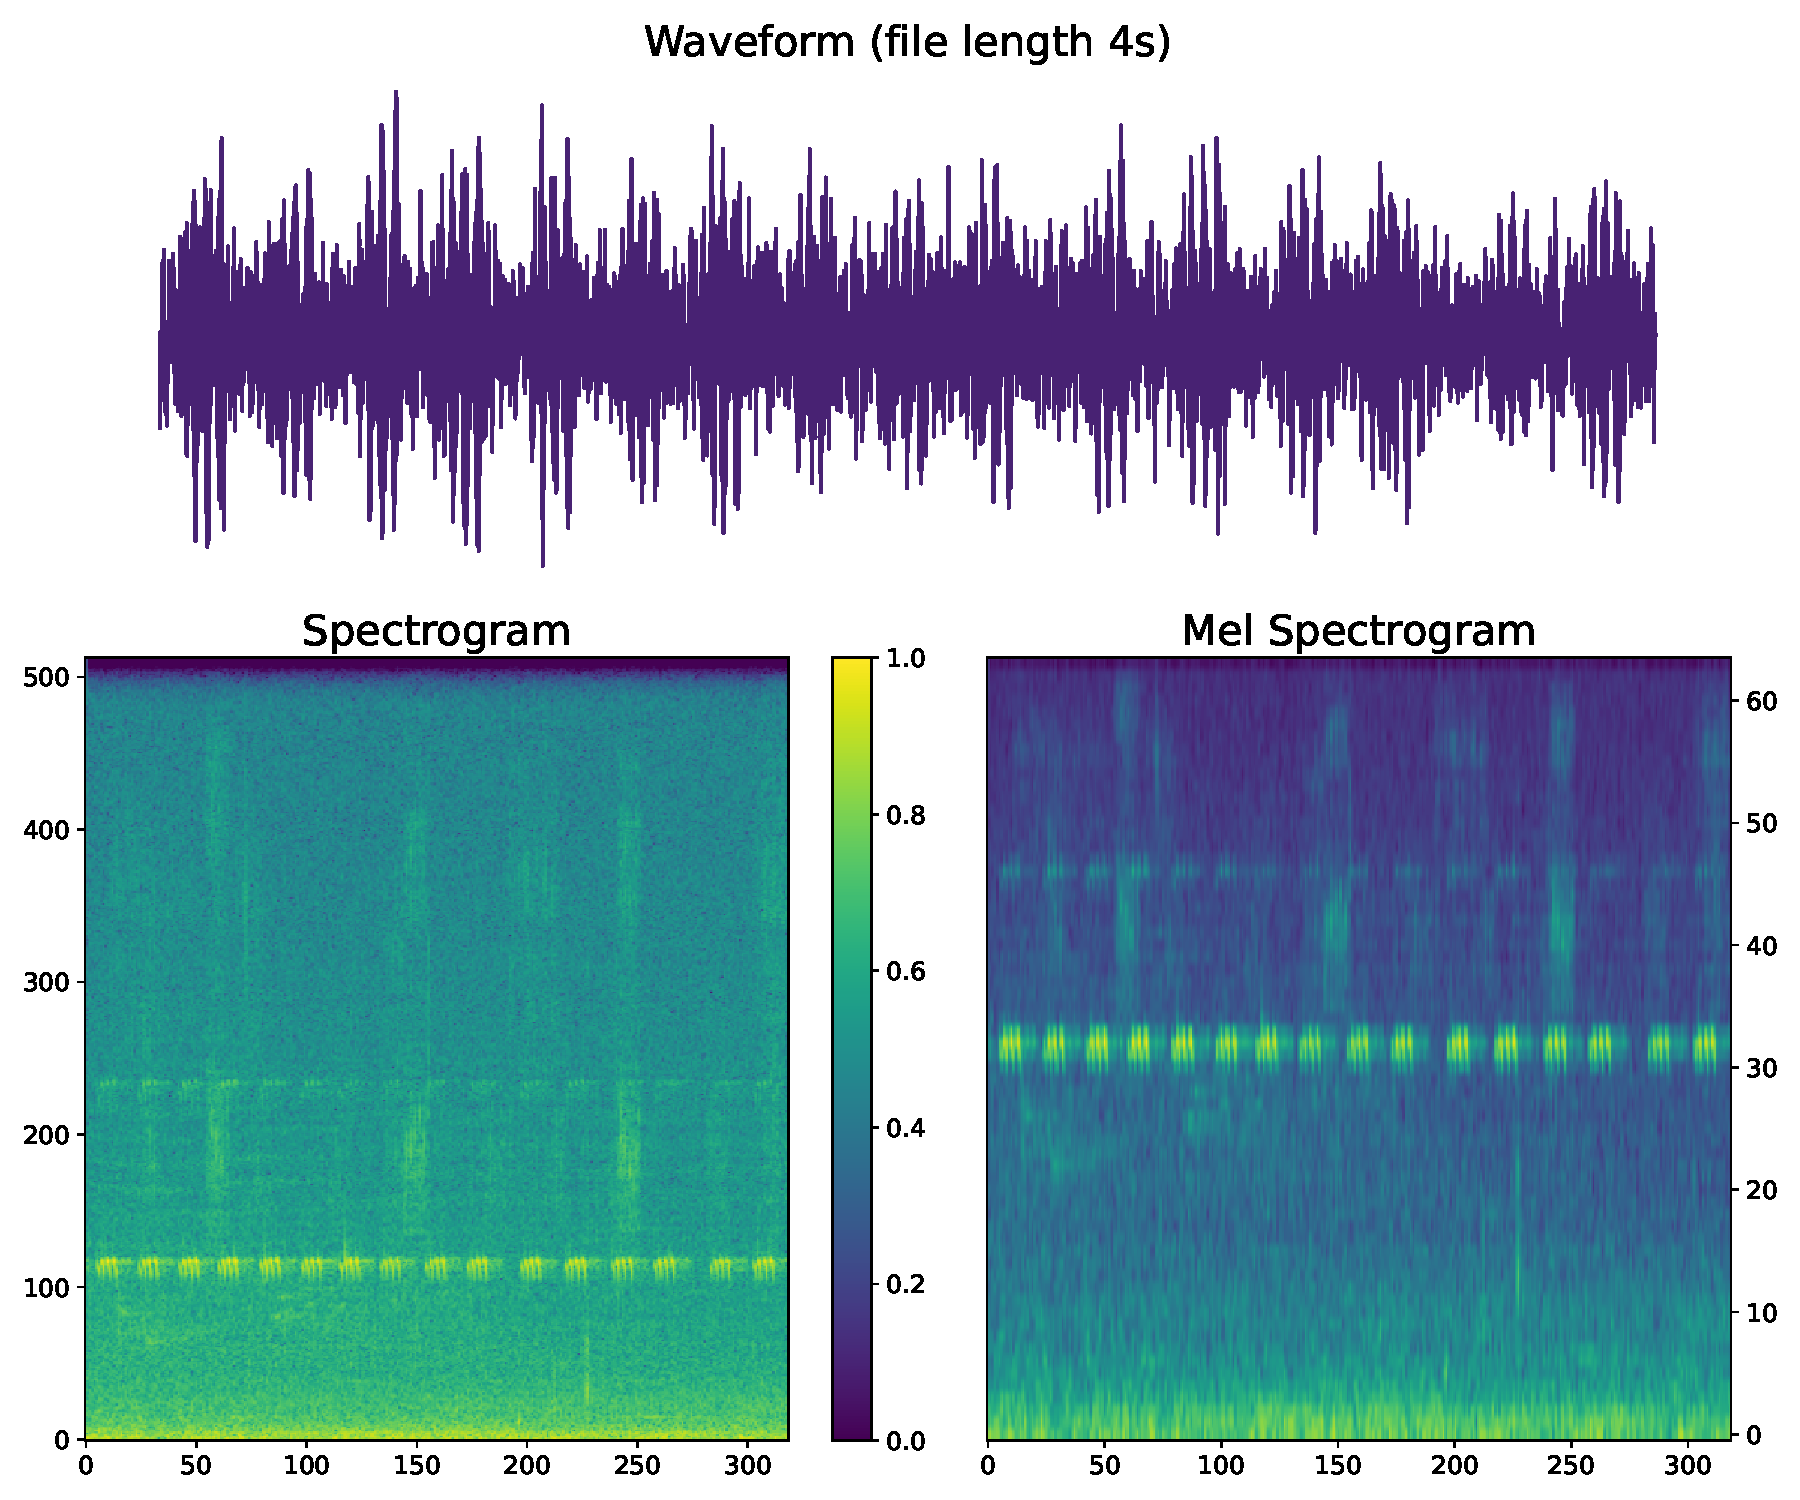
\includegraphics[width=0.85\textwidth]{figures/compare_spectrogram.pdf}
    \caption{Visualization of the two transformations of the audio signal.}
    \label{fig:1:transformations}
\end{figure}

To implement the two varieties of the transformation, the library torch and torchaudio where used.
A custom transformation method was implemented, that can be used as a layer in the model as shown in 
Listing \ref{lst:transformation}. Some of the parameters of the transformation where made configurable
and others dependant on them where calculated. In the hyperparameter tuning phase, the only parameter
that was tuned was the number of mel bins, which was set to either 64 to try the mel-spectrogram or -1
to use the standard spectrogram.

    \begin{lstlisting}[
        language=Python, 
        caption={Python code for the transformation of the audio signal}, 
        label={lst:transformation}]

    import torch
    import torchaudio

    class NormalizeSpectrogram(torch.nn.Module):
        def forward(self, tensor):
        return (tensor - tensor.min()) / (tensor.max() - tensor.min())

    normalize_transform = NormalizeSpectrogram()

    if n_mels == -1:
        spectogram = torchaudio.transforms.Spectrogram(
            n_fft=n_fft, 
            hop_length=int(n_fft/2), 
            win_length=n_fft)
    else:
        spectogram = torchaudio.transforms.MelSpectrogram(
            n_fft=n_fft,
            hop_length=int(n_fft/2),
            win_length=n_fft,
            n_mels=n_mels,
            f_max=self.sample_rate / 2)

    db_transform = torchaudio.transforms.AmplitudeToDB(top_db=top_db)

    self.transform = torch.nn.Sequential(
        spectogram, 
        db_transform, 
        normalize_transform)

    \end{lstlisting}








\subsubsection{Training}
% Describe the training process


\subsubsection{Evaluation}
% Describe the evaluation process


\subsection{Hyperparameter Tuning}